\documentclass[]{article}
\usepackage{lmodern}

\usepackage{graphicx,grffile}

\usepackage{xcolor} 
\usepackage{colortbl} 
\usepackage{longtable} 
\usepackage{relsize}
\usepackage{array}
\newcolumntype{L}[1]{>{\raggedright\let\newline\\\arraybackslash\hspace{0pt}}p{#1}}
\newcolumntype{C}[1]{>{\centering\let\newline\\\arraybackslash\hspace{0pt}}p{#1}}
\newcolumntype{R}[1]{>{\raggedleft\let\newline\\\arraybackslash\hspace{0pt}}p{#1}}




\usepackage{amssymb,amsmath}
\usepackage{ifxetex,ifluatex}
\usepackage{fixltx2e} % provides \textsubscript
\ifnum 0\ifxetex 1\fi\ifluatex 1\fi=0 % if pdftex
  \usepackage[T1]{fontenc}
  \usepackage[utf8]{inputenc}
\else % if luatex or xelatex
  \ifxetex
    \usepackage{mathspec}
  \else
    \usepackage{fontspec}
  \fi
  \defaultfontfeatures{Ligatures=TeX,Scale=MatchLowercase}
    \setmainfont[]{TeXGyrePagella}
\fi
\usepackage{tgpagella}
% use upquote if available, for straight quotes in verbatim environments
\IfFileExists{upquote.sty}{\usepackage{upquote}}{}
% use microtype if available
\IfFileExists{microtype.sty}{%
\usepackage{microtype}
\UseMicrotypeSet[protrusion]{basicmath} % disable protrusion for tt fonts
}{}
\usepackage[margin=1.3in]{geometry}
\usepackage{hyperref}
\hypersetup{unicode=true,
            pdftitle={RailCons CNL at Chalmers},
            pdfauthor={Bjørnar Luteberget},
            pdfborder={0 0 0},
            breaklinks=true}
\urlstyle{same}  % don't use monospace font for urls
\IfFileExists{parskip.sty}{%
\usepackage{parskip}
}{% else
\setlength{\parindent}{0pt}
\setlength{\parskip}{6pt plus 2pt minus 1pt}
}
\setlength{\emergencystretch}{3em}  % prevent overfull lines
\providecommand{\tightlist}{%
  \setlength{\itemsep}{0pt}\setlength{\parskip}{0pt}}
\setcounter{secnumdepth}{0}
% Redefines (sub)paragraphs to behave more like sections
\ifx\paragraph\undefined\else
\let\oldparagraph\paragraph
\renewcommand{\paragraph}[1]{\oldparagraph{#1}\mbox{}}
\fi
\ifx\subparagraph\undefined\else
\let\oldsubparagraph\subparagraph
\renewcommand{\subparagraph}[1]{\oldsubparagraph{#1}\mbox{}}
\fi

\title{RailCons CNL at Chalmers}
\author{Bjørnar Luteberget}
\date{2016-11-02}

\begin{document}
\maketitle

\section{\texorpdfstring{Formalizing ``Teknisk
regelverk''}{Formalizing Teknisk regelverk}}\label{formalizing-teknisk-regelverk}

The Norwegian railway authority has a comprehensive set of technical
regulations (``Teknisk regelverk'') for design/planning
(``prosjektering''), construction, and maintenance of railway
infrastructure. The text is also subdivided into 12 disciplines, such as
electric, track works, tunnels, and signalling.

\subsection{Goal}\label{goal}

The RailCons project would like to formalize relevant parts of the
technical regulations for use in the on-the-fly type of verification
which can be used within railway construction design software
(specifically the RailCOMPLETE software). This type of verification will
probably be limited to static infrastructure analysis, leaving the more
heavy-weight analysis of e.g.~the implementation of control systems to
specialized analysis software such as Prover AB (Sweden) or Systerel
(France). However, it could still be beneficial for the method for
formalizing the technical regulations to include more dynamic and
logically more complex kinds of information, as this could be used to
analyse the regulations in themselves, or as input to other types of
analysis software.

The suggested use cases are listed here by priority:

\begin{enumerate}
\def\labelenumi{\arabic{enumi}.}
\tightlist
\item
  On-the-fly verification inside the design tool for \textbf{static
  infrastructure}, probably based on the Datalog logic. Related
  sub-goals are:

  \begin{enumerate}
  \def\labelenumii{\arabic{enumii}.}
  \tightlist
  \item
    Engineers can understand what the verification engine is doing. (CNL
    + CAD)
  \item
    Produce reports on how/what is verified. (CNL + CAD with report
    generator)
  \item
    Regulations are changing, so regulations database needs to be
    maintained. (CNL editor)
  \item
    Expert knowledge, rules of thumb, local company knowledge base. (CNL
    editor)
  \end{enumerate}
\item
  Control system \textbf{implementation verification}, typically more
  computationally expensive, and based on other formalisms, such as
  timed automata, first order logic, etc.
\item
  Verification of human \textbf{activities and processes}, such as
  regulations for maintenance scheduling, or regulations for design
  \emph{considerations}. (For example, a non-standard design choice for
  infrastructure could be acceptable only when reasoning has been given
  for abandoning the standard choice.)
\item
  Analysis of the regulations in themselves, for example exposing
  inconsistencies.
\item
  Tranforming the regulations into a simpler, unambiguous text for human
  readers.
\end{enumerate}

\subsection{Regulations overview}\label{regulations-overview}

The technical regulations (\emph{``Teknisk regelverk''}) can be found at
\url{https://trv.jbv.no/} and consists of the following books:

\begin{itemize}
\tightlist
\item
  \textbf{Common regulations}: 501 Common regulations
\item
  \textbf{Common electrical}: 510 Design and construction
\item
  \textbf{Signs}: 515 Placement of signs along the track
\item
  \textbf{Superstructure (tracks)}: 530 Design, 531 Construction, 532
  Maintenance
\item
  \textbf{Substructure}: 520 Design and construction, 522 Maintenance
\item
  \textbf{Tunnels}: 521 Design and construction, 523 Maintenance
\item
  \textbf{Bridges}: 525 Design and construction, 527 Maintenance
\item
  \textbf{Overhead line}: 540 Design, 541 Construction, 542 Maintenance
\item
  \textbf{Low voltage and 22 kV}: 543 Design, 544 Construction, 545
  Maintenance
\item
  \textbf{Power supply}: 546 Design, 547 Construction, 548 Maintenance
\item
  \textbf{Signalling}: 550 Design, 551 Construction, 552 Maintenance,
  553 Assessment
\item
  \textbf{Telecommunications}: 560 Design and construction, 562
  Maintenance
\end{itemize}

Structure of each book:

\begin{itemize}
\tightlist
\item
  Each book repeats the \emph{common regulations} as the first three
  chapters.
\item
  Following this will typically be a \emph{general} section containing:

  \begin{itemize}
  \tightlist
  \item
    declaration of the scope of the book,
  \item
    references to relevant standards,
  \item
    definitions of relevant techincal terms,
  \item
    qualitative classifications, such as quality classes, risk classes,
    etc.
  \end{itemize}
\item
  The main part of a book consists typically of 5 to 10 chapters, each
  detailing a specific technical topic within the discipline. The text
  consists of:

  \begin{itemize}
  \tightlist
  \item
    Scope declarations
  \item
    Definitions
  \item
    Non-normative statements
  \item
    Comments
  \item
    Regulations (including tables and figures), with exceptions
  \item
    Examples
  \end{itemize}
\end{itemize}

\subsection{Scope and focus}\label{scope-and-focus}

The technical regulations contain a lot of generalities which are not
necessarily normative, nor directly useful in a design setting. Based on
the prioritized use case list, the following parts of the regulations
should be considered first in designing and testing the formalization
procedure:

\begin{enumerate}
\def\labelenumi{\arabic{enumi}.}
\tightlist
\item
  Superstructure design (track design / \emph{Overbygning: 530
  Prosjektering}), especially regulations and formulas regarding

  \begin{itemize}
  \tightlist
  \item
    track geometry: curvature, gradients, etc.
  \item
    switches: types, maximum speeds, naming (numbering), etc.
  \end{itemize}
\item
  Signalling design (\emph{Signal: 550 Prosjektering}), especially

  \begin{itemize}
  \tightlist
  \item
    signal placement, functions, sighting distance
  \item
    train detector placement, classification
  \item
    switch motors requirements and control system components
  \item
    automatic train protection system (ATC) placement and functions
  \item
    interlocking (control system) routes, conflicts, detection sections,
    safety classes, flank protection, overlaps, etc.
  \end{itemize}
\end{enumerate}

\section{Rule classification}\label{rule-classification}

This is an attempt to classify rule types, and could help determine what
the language needs to support, and how the railway language is
distinguished from other CNLs and general ontology languages.

\begin{itemize}
\item
  \textbf{Classes and properties}, descriptions of objects with
  (complex) classification and properties. Properties are typically

  \begin{itemize}
  \tightlist
  \item
    Picked from enumeration (enumerations defined by an ontology)
  \item
    Integers or floating point numbers
  \item
    String operations (not so important so far, not directly supported
    in Datalog).
  \end{itemize}

  See the RAINS CNL or any other ontology-based CNL.
\item
  \textbf{Formulas} mathematical type, usually also supported by
  ontology-like languages.
\item
  \textbf{Topology} specifies graph searches using the (somewhat
  expensive) built-in predicates such as \emph{connected},
  \emph{following}, \emph{between}, \emph{overlap}.
\item
  \textbf{Geometry} constraint language (as suggested by Gerardo).
\item
  \emph{Future:} \textbf{LTL/CTL} style model checking properties. Any
  examples of CNLs for this?
\item
  \emph{Future:}
\end{itemize}

Tables are not a class of rules, only syntactic sugar for facts.

\section{Translation}\label{translation}

The technique of controlled natural language will be investigated to
allow the input of regulations, especially those translatable into the
static infrastructure verification being developed in the RailCons
project.

\subsection{Non-textual information}\label{non-textual-information}

It could be beneficial to keep tables and figures from the regulations
when transitioning to the CNL, so that the CNL interfaces can use these
kinds of rich text.

Specifically, referring to figures and referring to the contents of
tables based on column and row headers, could be useful.

\subsection{Examples and relevance}\label{examples-and-relevance}

The following table lists some example excerpts from the regulations
along with a translation into English, and a comment about use cases and
relevance.

\newcommand{\tpar}[1]{ \multicolumn{5}{p{\textwidth}}{#1} \vspace{0.5em}}
\newcommand{\tparx}[1]{ \multicolumn{4}{p{\textwidth}}{#1} \vspace{0.5em}}


\begin{longtable}[h]{L{0.5cm} L{0.8cm} L{4.0cm} L{4.0cm} L{5.0cm}}
&Use cases &
Original text &
English translation &
Comments \\*
\hline \\*
\endhead
\tpar{ 
\textbf{Overbygning}: 530 Prosjektering, Kap. 8 Helsveist spor, 2.1.
} \\*
&\#4 &
De store krefter som kan forekomme i et helsveist spor stiller strenge krav til sporets konstruksjon. &
The large forces that may occur in a welded track makes stringent demands on the track construction.& 
This sentence is not normative, and is unlikely to have any use in automated verification.
\\
& & & & \\
\tpar{ 
\textbf{Overbygning}: 530 Prosjektering, Kap. 8 Helsveist spor, 2.1.3 a)
} \\*
&\#4 &
Ballasten skal på linjen og i hovedspor på statsjoner være fullverdig grovpukk (av størrelse 31.5 -- 63 mm) &
The ballast on the line and in the main track at stations must be purely coarse crushed stone  (size from 31.5 to 63 mm) &
This is a specification which is absolute, and rules out 
the need for specifying this as a part of the design, because
it is not part of a specific station.
It can still be valuable to support this sentence in a CNL, 
and in a formal representation.
\\
& & & & \\
\tpar{ 
\textbf{Overbygning}: 530 Prosjektering, Kap. 8 Helsveist spor, 2.1.2 a)
}\vspace{0.5em} \\* 
&\#1 &
Minste kurveradius for helsveist med betongsviller skal være 250 m. &
The lowest allowable radius of curvature for whole welded track on concrete sleepers is 250 m.& 
{This is a typical example of static infrastructure verification, expressible in Datalog as: \newline	
\footnotesize{
error(Segment) :- trackSegment(Segment), trackSegmentRadius(Segment, Radius), Radius < 250.
}
}
\\
& & & & \\
\tpar{ 
\textbf{Signal}: 550 Prosjektering, Kap. 6 Lyssignal, 2.1.2 j)
}\vspace{0.5em} \\* 
&\#1 &
Et innkjørhovedsignal skal plasseres $\geq$ 200 meter foran innkjørtogveiens første sentralstilte, motrettede sporveksel, se Figur 5. 
&
A home main signal shall be placed at least 200 m in front of the first controlled, facing switch in the entry train path (see Figure 5).
& 
{This is the example that we have been using most frequently for the RailCons verification tool. Datalog:\newline
\footnotesize{
error(Sig,Sw) :- firstFacing(Bdry, Sw, Dir), homeSignalBetween(Sig, Bdry, Sw), distance(Sig, Sw, Dir, L), L < 200.
}
}
\\
& & & & \\

\tpar{ 
\textbf{Signal}: 550 Signal, Kap. 5 Forriglingsutrustning, 2.8.1 Dekningsgivende objekt
}\vspace{0.5em} \\* 
&\#1, \#2 &
Følgende objekt kan være dekningsgivende: Hovedsignal, Dvergsignal, Sporveksel, Sporsperre, Avsporingstunge, Signal E35 Stoppskilt.
Et hovedsignal skal vise signal ”Stopp” for å være dekningsgivende.
&
The following objects can provide flank protection: main signal, shunting signal, switch, derailer, derailing tongue, signal E35 stop sign.
A main signal must display "stop" to provide flank protection.
&
This regulation is relevant both for \textbf{specifying} the control system, and for verifying the \textbf{implementation}. The specification chooses which objects to use for flank protection (\textbf{static}) and what state they can be used in, while the implementation must correctly enforce the conditions saying which message the signal displays (\textbf{dynamic}).
\\
& & & & \\
\tpar{ 
\textbf{Signal}: 550 Prosjektering, Kap. 6 Lyssignal, 2.1.2 i)
}\vspace{0.5em} \\* 
&\#1, \#3 &
Et hovedsignal bør ikke plasseres i tunneler, på bruer, eller andre steder hvor en eventuell togstans og dermed muligheten for avstigning, vil medføre fare. 
&
A main signal should not be placed in tunnels, on bridges, or other places where halting trains and thus the possibility of disembarking, can impose dangers.
& 
Here we have an example of a ``\emph{should}'' modality, where the 
static infrastructure verification could issue a warning, but not an error. 
Also, it could be required to document the alternatives that were considered
when deciding on the design.
\\
& & & & \\
\tpar{ 
\textbf{Signal}: 550 Prosjektering, Kap. 5 Forriglingsutrustning, 4.1.1.1 i)
}\vspace{0.5em} \\* 
&\#2 &
For at en togvei skal kunne fastlegges, skal et objekt som gir dekning til togveien være dekningsgivende. 
&
For a train route to be deactivated, any object giving flank protection must be in a protecting state.
& 
This regulation concerns only the state of the control system, and as such 
relates to the implementation of the control system and not the static infrastructure specification.
\\
& & & & \\ 
& & & & \\ 
& & & & \\ 
\tpar{ 
\textbf{Overbygning}: 530 Prosjektering, Kap. 5 Sporets trasé, 3.1 Dimensjonerende parametre
} \\*
& \#1 & 
See table below.
& (a) minimum radius, (b) maximal superelevation, 
(c) limit on superelevation cause by derailment risk at low speeds,
(d) limit for superelevation rate of change,
(e) limit for superelevation deficit.
&
Limiting values are organized in a table for use in formulas in other sections.
\\*
&\tparx{
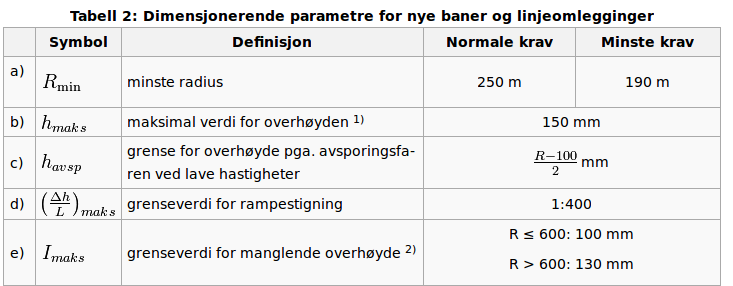
\includegraphics[width=0.9\textwidth]{tabless.png}
} 
\\
& & & & \\
\tpar{ 
\textbf{Overbygning}: 530 Prosjektering, Kap. 5 Sporets trasé, 3.7 Sporveksler og sporforbindelser
} \\*
& \#1 & 
Avstanden mellom sporveksel og overgangskurve, sirkelkurve, bru eller annen motstående sporveksel skal ikke være mindre enn avstanden M gitt i \emph{Kurver uten overgangskurver}, krav b). M skal imidlertid ikke være kortere enn 6 m. 
& 
The distance between the switch point and the transition curve, circle curve, bridge or other opposite switch point should not be less than the distance M given in section \emph{``curves without transition curves''}, requirements b). M shall not be shorter than 6 m.
&
The parameter $M$ is explained by the figure below. Reference is given to 
another section of the regulations.
\\*
&\tparx{
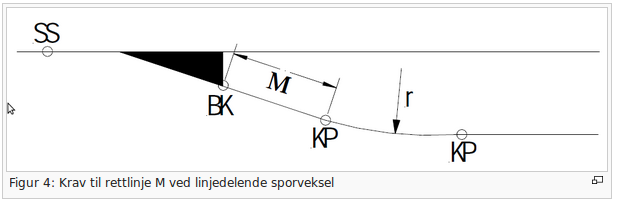
\includegraphics[width=0.8\textwidth]{figuress.png}} \\
& & & & \\
\tpar{ 
\textbf{Overbygning}: 530 Prosjektering, Kap. 5 Sporets trasé, 5 Største hastighet -- sporets geometri
} \\*
& \#1 & 
Hastigheten i en kurve skal ikke være større enn:
{\footnotesize
\begin{equation*}
V = 0,291 \cdot\sqrt{R\left(h +I_{\text{maks}}\right)}\quad \text{(5)}
\end{equation*}
}
Hvis ligning 5 i tilfeller med falsk overhøyde gir lavere verdi enn 20 km/h gjelder $V = 20$ km/h.
&
The speed in a curve shall not exceed:
{\footnotesize
\begin{equation*}
V = 0,291 \cdot\sqrt{R\left(h +I_{\text{maks}}\right)}\quad \text{(5)}
\end{equation*}
}
If Eq. 5 gives a lower value than 20 km/h in situations with false superelevation, then $V = 20$ km/h shall be used.
& 
Use of equations with designed and given parameters.\\
& & & & \\
\tpar{ 
\textbf{Signal}: 552 Vedlikehold, Kap. 6 Lyssignal, 3 Lyssignaler
} \\*
& \#3, \#4 & 
Dersom lyssignal er vridd eller på annen måte kommet ut av stilling skal dette utbedres snarest. 
&
If a signal is twisted or in other ways are out of position, this shall be fixed as soon as possible.
& 
Typical maintenance regulation. Here, it might be sufficient to identify this as a \emph{checklist item}, for 
maintenance scheduling and reporting purposes.
\end{longtable}


\section{Translation toolchain}\label{translation-toolchain}

Suggest the following steps in transferring \emph{teknisk regelverk}
into Datalog.

\begin{enumerate}
\def\labelenumi{\arabic{enumi}.}
\item
  \textbf{Original}: \emph{Teknisk regelverk} in its original form
\item
  \textbf{Categorization}: Non-automatic or assisted transfer from
  original text to a categorization of each part (sentence?) of the text
  into the following:

  \begin{itemize}
  \tightlist
  \item
    Definitions
  \item
    Scopes
  \item
    Rules
  \item
    Figures
  \item
    Tables
  \end{itemize}
\item
  \textbf{High level CNL}: Non-automatic or assisted transfer of the
  definitions and rules in the categorized text into a high-level CNL,
  with Norwegian-like and/or English-like concrete syntax, supporting
  the kind of modalities and logic in the target (Datalog) language,
  with special constructs for the railway domain.
\item
  \textbf{Low-level CNL}: Fully automatic transfer from the high-level
  CNL into a format which is specially suited for transfer to Datalog.
  Rules can be in the following form:

\begin{verbatim}
Given "FACT_1" and "FACT_2" ..., then
"COND_1" and "COND_2" ..., should be satisfied.
\end{verbatim}
\item
  \textbf{Datalog}: final output format of the translation
\end{enumerate}

\subsection{High level CNL}\label{high-level-cnl}

The high level CNL should:

\begin{itemize}
\tightlist
\item
  have Norwegian-like and/or English-like concrete syntax,
\item
  recognize several types of top-level sentence types:

  \begin{itemize}
  \tightlist
  \item
    definition, obligation, constraint, suggestion, heuristic, etc.
  \end{itemize}
\item
  allow logic which is easily translatable to the target (Datalog)
  language

  \begin{itemize}
  \tightlist
  \item
    conjunction, negation, arithmetic, implication(?)
  \end{itemize}
\item
  support special constructs for the railway domain.
\end{itemize}

\subsubsection{Top-level sentence types}\label{top-level-sentence-types}

Several kinds of sentences:

\begin{itemize}
\item
  \textbf{Definition} defines something which can be referred to by
  other sentences. Example:

\begin{verbatim}
The minimum radius R_min for use in formulas is 200 m.
\end{verbatim}
\item
  \textbf{Obligation} is a
\item
  \textbf{Constraint} is an absolute demand, possibly on the static
  infrastructure. Example:

\begin{verbatim}
The minimum radius for any track on a new station is R_min.
\end{verbatim}
\item
  \textbf{Suggestion} is a \emph{``should''} statement.

\begin{verbatim}
A main signal should not be placed in tunnels.
\end{verbatim}
\item
  \textbf{Heuristic} might be used to give a suggestion for missing
  information, but should not override any specified information.
\item
  \textbf{Comments} are maybe not worth representing?
\end{itemize}

\subsubsection{Low-level logic}\label{low-level-logic}

The top-level sentence types define which parts the sentence is made up
of, while the low-level logic can be

\begin{itemize}
\item
  \textbf{Conjunction}, example:

\begin{verbatim}
A signal shall belong to a track and have a direction.
\end{verbatim}
\item
  \textbf{Negation}, example:

\begin{verbatim}
A signal shall not be taller than 9 m.
\end{verbatim}
\item
  \textbf{Arithmetic}:
\item
  \textbf{Implication}.
\end{itemize}

\subsubsection{Railway constructs}\label{railway-constructs}

To give more natural-ness to sentences, a vocabulary of railway terms
will be ``baked in'' to the language. Some suggestions:

\begin{itemize}
\item
  Any object type known in the object model for static infrastructure
  should be a recognized \emph{noun} in the natural language, and the
  presence an instance of this noun (\texttt{a\ signal}) is translated
  into an ``individual'' with the corresponding classification. I.e.,
  \texttt{a\ signal} will be translated into the unary predicate
  \texttt{signal(}\(\__0\)\texttt{)} in the final representation.
\item
  Known relations should be complemented with specific natural language,
  such as:

  \begin{itemize}
  \item
    \texttt{distance(a,b,l)}

    ---\textgreater{} \texttt{the\ distance\ from\ a\ to\ b\ is\ l}
  \item
    \texttt{distance(a,b,l),\ l\ \textless{}\ 50}

    ---\textgreater{}
    \texttt{the\ distance\ from\ a\ to\ b\ is\ less\ than\ 50\ m}
  \item
    \texttt{track(X)}

    ---\textgreater{} \texttt{X\ is\ a\ track} (for any known object
    type)
  \item
    \texttt{track(X),\ trackQualityClass(X,A)}

    ---\textgreater{} \texttt{X\ is\ a\ track\ of\ quality\ class\ A}
  \item
    \texttt{boundary(B),\ firstSameDirSwitch(B,Sw),\ facingSwitch(B,Sw),\ controlled(Sw)}

    ---\textgreater{}
    \texttt{The\ first\ facing,\ controlled\ switch\ after\ a\ station\ boundary}
  \end{itemize}
\end{itemize}

\subsubsection{Other natural-ness
considerations}\label{other-natural-ness-considerations}

\begin{itemize}
\item
  Reflection from facts to conditions, for example:

  \begin{itemize}
  \tightlist
  \item
    \texttt{If\ X\ is\ a\ track\ with\ quality\ class\ A,\ then\ X\ must\ have\ a\ radius\ higher\ than\ 500\ m\ in\ all\ segments}
  \end{itemize}

  is written as

  \begin{itemize}
  \tightlist
  \item
    \texttt{Tracks\ of\ quality\ class\ A\ must\ have\ radius\ higher\ than\ 500\ m\ in\ all\ segments}
  \end{itemize}
\item
  From the GF book, chapter 6, semantic actions:

  \begin{itemize}
  \item
    \emph{Anaphroric} expressions:

\begin{verbatim}
If a man walks he talks
\end{verbatim}
  \item
    \emph{Aggregation} transfer:

\begin{verbatim}
John runs or John walks --> John runs or walks
\end{verbatim}
  \end{itemize}
\item
  From the GF book, chapter 8, interfacing formal and natural languages:

  \begin{itemize}
  \tightlist
  \item
    Natural language generation to/from logic can in general require
    steps that are outside of the grammar. However, some possibilities
    exist for improving naturalness using GF directly.
  \end{itemize}
\end{itemize}

The fact that Datalog disallows nested predicates (function symbols),
simplifies some aspects of linearization into natural language. For
example, the negation of arbitrary sentences (as presented on p.~190 in
the GF book) is not necessary, as negation is only possible in body
literals, which cannot be nested. More specifically, since literals can
have the clause type \texttt{Cl} instead of the sentence type
\texttt{S}, natural expressions of negation are available directly from
the resource grammar.

Whenever negation required over a complex term is needed, it is required
to define an intermediate Datalog predicate whose atomic representation
can be negated instead of the complex. This avoid the (usually less
elegant) sentence construction ``it is not the case that \ldots{}''.

These considerations have led to the comparison section below.

\subsection{Modules}\label{modules}

This is the current structure of the RailCNL GF grammar.

\begin{itemize}
\item
  RailCNL (main)
\item
  Datalog
\item
  Ontology

  \begin{itemize}
  \tightlist
  \item
    Classes
  \item
    Properties (=, != \textless{}, \textgreater{})
  \item
    Combine these into selections (subject, object, condition)
  \item
    Constr./obl./rec. that selections have properties.
  \end{itemize}
\item
  Graph

  \begin{itemize}
  \tightlist
  \item
    All/exists path from SEL to (first) SEL must/should pass SEL (SEL is
    a selection from the Ontology grammar)
  \item
    Distance from SEL to SEL must be RESTR
  \end{itemize}
\end{itemize}

\subsubsection{Other modules/features}\label{other-modulesfeatures}

Further grammar support could include the following.

\begin{itemize}
\item
  Object placement

  \begin{itemize}
  \tightlist
  \item
    On bridge, in tunnel, etc.
  \item
    ``Where freight trains brake''
  \end{itemize}
\item
  Sighting
\item
  Static driving constraints

  \begin{itemize}
  \tightlist
  \item
    Must not pass more than 4 balise groups per second (Define static
    velocities (sign, atc, max static, max dynamic))
  \item
    Safety zones, residual energy, potential consequences
  \end{itemize}
\item
  Track design
\item
  Constructions (geometry)

  \begin{itemize}
  \tightlist
  \item
    Platforms (relate signalling to constructions)
  \item
    ``Things in the way''.
  \end{itemize}
\item
  Catenary design (+ return power, grounding/earthing)
\item
  Availability, robustness in components
\end{itemize}

\subsection{Strategies for translating HL to
LL}\label{strategies-for-translating-hl-to-ll}

The \textbf{low level} (LL) language has a grammar which is close to
Datalog, adding only the distinction between rules (definition,
constraint, etc.), and metadata about rules (name, ID, extended
description, severity, etc.), which was organized as \emph{structured
comments} in the prototype (from iFM). It linearizes either directly to
Datalog, or to a (somewhat less natural) CNL.

The \textbf{high level} (HL) language adds constructs as described in
the sections above. The translation from HL language to LL language
should be deterministic.

A few strategies have come to mind:

\subsubsection{Basic GF resource grammar
use}\label{basic-gf-resource-grammar-use}

\begin{itemize}
\tightlist
\item
  CNL :
  ``\texttt{if\ X\ is\ a\ macroscopic\_node,\ then\ X\ is\ a\ station\_boundary}''.
\item
  Write resource grammar linearization (natural language AST is only
  implicit).
\item
  AST : ``\texttt{ifthen(macroscopic\_node(X),station\_boundary(X)).}''
\end{itemize}

It is not directly possible to make variables implicit in this approach.
(From chapter 8 of the GF book: \emph{Natural language generation
to/from logic can in general require steps that are outside of the
grammar.})

\subsubsection{Montague grammars in GF}\label{montague-grammars-in-gf}

Approach described in \emph{Aarne Ranta, ``Computational Semantics in
Type Theory''}.

\begin{itemize}
\item
  CNL : ``\texttt{all\ women\ walk}''.
\item
  Use resource grammar to convert sentence into natural language AST
  (explicit resource grammar AST).

  \texttt{Cl(Pred\ VP\ (Det\ CN\ woman\_N\ {[}....{]}))}
\item
  Use a transfer function to \emph{interpret} the sentence into a logic.
  \texttt{All\ (\textbackslash{}x\ -\textgreater{}\ If\ (iN\ woman\_N\ x)\ (iV\ walk\_x)).}
\end{itemize}

Requires higher-order types in GF, and writing a transfer function. Not
necessarily a two-way approach.

\subsubsection{AST transfer functions}\label{ast-transfer-functions}

Generalizing the above.

\begin{itemize}
\item
  HL CNL :
  ``\texttt{A\ macroscopic\ node\ is\ {[}also{]}\ a\ station\ boundary.}''.
\item
  Write an AST and resource grammar linearization which supports all of
  the interesting constructs. Here:

  \texttt{SubClass(NounModifier(macroscopic,\ node),\ NounModifier(station,\ boundary)).}
\item
  Write transfer functions from HL to LL, optionally back again.

  \texttt{macroscopic\_node(X)\ -\textgreater{}\ station\_boundary(X).}
\item
  Linearize to LL.
\end{itemize}

\subsubsection{AST rewriting system}\label{ast-rewriting-system}

Converting from LL to HL might be complicated. Straight-forwardly
writing an explicit transfer function from LL to HL might not be
feasible. Also, if we consider the HL grammar an (extensible) extension
of the LL grammar, then there might be several \emph{stages of
refinement} going from the LL language to the HL language. These factors
suggest that a term rewriting system (rule-based) might be suitable. In
this case, we should be able to show that the LL language is a normal
form.

It might not be a top priority to convert from LL to HL, but it could
also be used to illustrate how extending the HL with better constructs
improves the naturalness of the language.

See \emph{Ranta: Translating between language and logic} for an overview
of rewriting rules used in a first order logic natural language
generation system, going from the low level logic representation to a
higher level AST which generates more natural sentences.

\section{Sentence translation case
studies}\label{sentence-translation-case-studies}

\subsection{Object type constraints}\label{object-type-constraints}

Let's start with the following equivalent sentences:

\begin{itemize}
\item
  Datalog:

  \texttt{error\_trackquality(X)\ :-\ track(X),\ !trackQualityClass(X,k0)}.
\item
  Low level, in Datalog style

\begin{verbatim}
<constraint id="trackquality" params="X">
   track(X), !trackQualityClass(X,k0)
</constraint>
\end{verbatim}
\item
  Low level, in CNL style

\begin{verbatim}
<constraint id="trackquality" params="X">
   Given {X is a track}, then
   {quality class of X is k0} should be satisifed.
</constraint>
\end{verbatim}
\item
  High level CNL could be any of these:

  \begin{itemize}
  \tightlist
  \item
    \texttt{For\ any\ track\ X,\ the\ quality\ class\ of\ X\ must\ be\ k0}
  \item
    \texttt{All\ tracks\ must\ have\ quality\ class\ k0}.
  \item
    \texttt{Every\ track\ must\ have\ quality\ class\ k0}.
  \item
    \texttt{A\ track\ shall\ have\ quality\ class\ k0}.
  \item
    \texttt{A\ track\ must\ have\ quality\ class\ k0}.
  \end{itemize}
\end{itemize}

A structure (AST) for this constraint could be

\begin{verbatim}
   Constraint = Constraint [Clause] [Clause].
   Clause = Clause Predicate [Parameter].
   Predicate = Predicate String.
   Parameter = Constant String | Variable String.
   
\end{verbatim}

The actual abstract representation we want to express is then the
following:

\begin{verbatim}
   Constraint [Clause (Predicate "track") [Variable "X"]] 
              [Clause (Predicate "trackQualityClass") [Variable "X", Constant "k0"]]
\end{verbatim}

Instead of the very general ``\emph{predicate}'', we could instead use
classification, property, association, etc. primitives, so that we get
something like:

\begin{verbatim}
   Constraint [Class "track" (Variable "X")] 
              [Property "qualityClass" (Variable "X") (Constant "k0")]
\end{verbatim}

This could maybe help to restrict predicates to one and two parameters
for user-defined concepts, while allowing special internally defined
predicates, like \emph{distance}, \emph{between}, etc. to have natural
linearizations. This could be achieved through specialization of the
grammar for these concepts, instead of supporting arbitrary higher-arity
relations.

\subsection{Other examples}\label{other-examples}

\subsubsection{Classification}\label{classification}

\begin{verbatim}
 A *macroscopic node* is considered a *station boundary*.
\end{verbatim}

\subsubsection{Definition (search)}\label{definition-search}

\begin{verbatim}
 A *default train route* consists of two main signals Sa and Sb, 
 both oriented in the direction Dir, such that Sb follows Sa and
 there is a path without signals from Sa to Sb in direction Dir.
\end{verbatim}

\subsubsection{Object properties}\label{object-properties}

\begin{verbatim}
 All signal should have a type. / Alle signaler skal være av en signaltype.
 
\end{verbatim}

\subsubsection{Must placement}\label{must-placement}

The placement of the word must in the sentence determines where the
subject ends and the condition starts. Moving it also affects the number
of rules that must be generated.

Examples:

\begin{itemize}
\item
  \emph{If a track has closest balise, the balise must be red.}

\begin{verbatim}
track(X), balise(A), closest_balise(X,A), !red(A) -> error
\end{verbatim}
\item
  \emph{All tracks must have a closest balise which is red.}

\begin{verbatim}
track(X), balise(A), !closest_balise(X,A)          -> error

track(X), balise(A),  closest_balise(X,A), !red(A) -> error
\end{verbatim}
\item
  \emph{A track which has a closest balise which is red, must exist.}

\begin{verbatim}
!track(X) -> error

track(X), balise(A), !closest_balise(X,A) -> error

track(X), balise(A), closest_balise(X,A), !red(A) -> error
\end{verbatim}
\end{itemize}

All of these examples also requires the (graph-domain) definition of
\texttt{closest\_balise}.

\subsubsection{And/or and negation}\label{andor-and-negation}

The condition part of a sentence is negated in the rule. As Datalog does
not (necessarily) have an \emph{or} operator, nor negation over complex
terms, these must be given special consideration.

\begin{itemize}
\item
  \emph{Et hovedsignal bør ikke plasseres i tunneler eller på broer.}

\begin{verbatim}
Heuristic (Property (Class Signal) (Adjective Main)) 
  (Not (Or (Placement Tunnel) (Placement Bridge)))

signal(X), type(X,main), placement(X,tunnel) -> warning
signal(X), type(X,main), placement(X,bridge) -> warning
\end{verbatim}
\item
  \emph{Et hovedsignal bør festes i mast eller åk.}

\begin{verbatim}
Heuristic (Property (Class Signal) (Adjective Main)) 
  (Or (Mounting Mast) (Mounting Yoke))

signal(X), type(X,main), !should_mounting_rule123(X) -> warning
mounting(X, mast) -> should_mounting_rule123(X).
mounting(X, yoke) -> should_mounting_rule123(X).
\end{verbatim}
\end{itemize}

\section{System overview}\label{system-overview}

A verification and knowledge base editor system integrated

\begin{itemize}
\tightlist
\item
  Basic low-level grammar (GF, static)
\item
  Ontology / vocabulary based on railML or RailCOMPLETE config, from C\#
  classes, XSD or OWL ontology or similar. (could be static)

  \begin{itemize}
  \tightlist
  \item
    Could be extended with CNL-related information such as noun genders.
  \end{itemize}
\item
  High-level grammar extensions (GF, static)

  \begin{itemize}
  \tightlist
  \item
    Ontology (classes and properties)
  \item
    Graph searches (``first'', ``all paths'', ``some paths'', etc.)
  \end{itemize}
\item
  Dynamically defined concepts.
\item
  Dynamic evaluation/testing environment.
\end{itemize}

\subsection{Dynamic}\label{dynamic}

In the KeY book chapter by Johannisson, it seems that he has used a
conversion from UML to GF, then the GF compiler, and combined this with
the static part of the grammar.

We would like to avoid using the GF compiler dynamically from the
interactive knowledge base system, for the following reasons.

\begin{itemize}
\tightlist
\item
  Recompilation of grammar with new concepts might be required very
  often, for example after adding a definition. An actually dynamic
  vocabulary in the PGF runtime library seems more fitting.
\item
  GF compiler is a heavier dependency for the engineering tool than the
  PGF library alone.
\item
  GF compiler distribution has license incompatibility with
  RailCOMPLETE.
\end{itemize}

Hopefully, this functionality is covered by C runtime PGF library
\emph{proper noun callbacks}.

\pagebreak

\section{RailCOMPLETE (.NET)
integration}\label{railcomplete-.net-integration}

Some consideration for integrating a GF CNL into a .NET desktop
application without to many heavy dependencies.

\begin{enumerate}
\def\labelenumi{\arabic{enumi}.}
\item
  We need to distribute our application in executable form. As we are
  not using Haskell in the RailCOMPLETE software, Haskell libraries
  would be a heavy dependency. We will focus instead on the C runtime,
  and assume that the C runtime has the same capabilities as the Haskell
  runtime. At least when disregarding higher-order and dependent types,
  this seems to be the case. The C runtime has been used in other
  projects with platform integrations.
\item
  The C runtime compiles with autotools and GCC. These are available on
  Windows through MinGW. I am having a bit of trouble to find out
  exactly what MinGW libraries must be distributed together with an
  application, and would prefer to also eliminate this dependency by
  using the Microsoft (MSVC) compiler. I managed to do a port the GF
  runtime to CMake and MSVC, which is not entirely trivial because (a)
  the code uses some GCC-specific extensions of C, and (b) the MSVC
  doesn't fully support the C99 standard, and (c) exporting functions
  and data from a library is slightly different on Windows. Some code
  changes were required, but the result was a very lightweight library
  (a few hundred kB). I can later clean this up and offer it to the GF
  developers, if they are willing to pollute the code with some
  MSVC-specific workarounds.
\item
  A .NET wrapper library is required to do a practical/idiomatic and
  safe (in terms of memory/resources) interface to the C library. The
  Python and Java wrappers show how to do this, but the Python wrapper,
  for example, is 3000 lines of C code, which could require a bit of
  effort to port. I have started on this, and it seems to be doable in a
  few days work, especially if some features can be (temporarily)
  omitted.
\item
  Manipulation of the AST and passing the AST from the library to the
  application code, is done through strings. To have type-safe
  manipulations, the GF compiler can generate Haskell code which
  transforms the strings into a Haskell algebraic data type. A wrapper
  library in another language should have something similar if it aims
  to manipulate a specific application grammar, which we want to do.
  Python (and Java?) wrappers lack this, it seems, and use instead a
  general data type for expressions. Maybe applications in these
  languages are more geared towards treating grammars in general, not
  specific application grammars.
\end{enumerate}

\pagebreak

\section{Schedule}\label{schedule}

\begin{itemize}
\tightlist
\item
  \textbf{1 Nov - 14 Dec} Learn GF, make LL CNL, start on HL CNL, before
  Dec 14, when John takes parental leave.
\item
  \textbf{1 Jan - 1 Feb} Work with Gerardo when he is back after new
  year, on the assumptions about logic in the verification (Datalog).
\item
  \textbf{Feb 2017?} When CNL is well under way, start exploring

  \begin{itemize}
  \tightlist
  \item
    Regulations which need more than Datalog, e.g.~SAT solving.
  \item
    Synthesis/constraint solving for railway signalling design.
  \end{itemize}
\item
  \textbf{Mar 2017} Write paper for suitable publication venue. Gerardo
  will look for possibilities.
\end{itemize}

\pagebreak

\section{Literature list and links}\label{literature-list-and-links}

\subsection{CNL}\label{cnl}

\begin{itemize}
\tightlist
\item
  Thomas Kuhn survey
\item
  Aarne Ranta, Computational semantics in type theory - Mathématiques et
  sciences
\item
  Hähnle, Johannisson, Ranta, An Authoring Tool for Informal and Formal
  Requirements Specification
\item
  Burke, Johannisson, Translating Formal Software Specifications to
  Natural Language
\item
  Ranta: translating between logic and language
\item
  Key Book chapter by Johannisson
\item
  Bringert, Ranta: A pattern for almost compositional functions
\end{itemize}

\subsection{Applications}\label{applications}

\begin{itemize}
\tightlist
\item
  Emani: An approach for automatic formalization of business rules
\end{itemize}

\subsection{GF}\label{gf}

\begin{itemize}
\item
  Web page

  \url{http://www.grammaticalframework.org/}
\item
  Library synopsis

  \url{http://www.grammaticalframework.org/lib/doc/synopsis.html}
\item
  MOLTO application grammar building (``best practices'')

  \url{http://www.molto-project.eu/sites/default/files/MOLTO_D2.3.pdf}
\item
  PhD thesis of Krasimir Angelov
\end{itemize}

\subsection{Tools}\label{tools}

\begin{itemize}
\item
  Minibar

  \url{http://cloud.grammaticalframework.org/minibar/minibar.html}
\item
  Syntax editor (tree / linear)

  \url{http://cloud.grammaticalframework.org/syntax-editor/editor.html}
\item
  CSE-ID splits sentences (shallow parsing)

  \url{http://ad-wiki.informatik.uni-freiburg.de/research/Projects/CSDIE}
\item
  Illinois chunker also splits sentences (shallow parsing)

  \url{https://cogcomp.cs.illinois.edu/page/software_view/Chunker}
\item
  Stanford parser gives complete parses

  \url{http://nlp.stanford.org/}
\end{itemize}

\pagebreak

\section{Other notes}\label{other-notes}

\subsection{Why don't we store the syntax tree instead of the source
code?}\label{why-dont-we-store-the-syntax-tree-instead-of-the-source-code}

\url{http://softwareengineering.stackexchange.com/questions/119095/why-dont-we-store-the-syntax-tree-instead-of-the-source-code}

\begin{itemize}
\tightlist
\item
  Requiring strict correspondence of AST and concrete syntax loses
  whitespace, comments, meaningful formatting, etc.
\item
  Half-written code or almost-correct code is meaningful to the human
  reader, but the AST representation is not meaningful at all.
\item
  No two languages are perfect matches.
\end{itemize}

\subsection{Editor ideas}\label{editor-ideas}

\begin{itemize}
\item
  Outer/inner editor: the regulations might require structuring in
  larger documents, while we would like to keep the CNL editor on a
  sentence-scale.

  See \url{https://clearly.pl/tutorial/}
\end{itemize}

\end{document}
